%\documentclass[10pt]{report}
%\usepackage{epsf}
%\usepackage{amsmath}
%\usepackage{amssymb}
%\usepackage{palatino}
%\usepackage[dvips]{graphics}
%\usepackage{fancyhdr}
%\usepackage{epsfig}
%\usepackage{multirow}
%\usepackage{cancel}
%\parindent 0in
%\parskip 1ex
%\oddsidemargin  0in
%\evensidemargin 0in
%\textheight 8.5in
%\textwidth 6.5in
%\topmargin -0.25in

%\pagestyle{fancy}
\fancyhead[LO]{\bf BME354L - Palmeri - Spring 2013}
\fancyhead[RO]{{\bf Second-Order Systems}}
\fancyfoot[C]{This work is licensed under a Creative Commons Attribution 3.0 Unported License.}

\documentclass[10pt]{article}
\usepackage{wrapfig}
%\usepackage{epsf}
\usepackage{fancyhdr,epsfig,graphics,tabularx,times}
\usepackage{amsmath}
\usepackage{amssymb}
\usepackage{palatino}
%\usepackage[dvips]{graphics}
\usepackage{fancyhdr}
\usepackage{epsfig}
\usepackage{multirow}
\usepackage{cancel}
\usepackage[bookmarks]{hyperref}
\usepackage{longtable}
\usepackage{soul}
\parindent 0in
\parskip 1ex
\oddsidemargin  0in
\evensidemargin 0in
\textheight 8.5in
\textwidth 6.5in
\topmargin -0.25in
\setcounter{section}{0}

\pagestyle{fancy}
\lhead{\bf BME354L: Introduction to Medical Instrumentation}
\rhead{\bf Nightingale (Spring 2015)}
\cfoot{\thepage}



\begin{document}
\section*{Review - Second Order Systems}

 \begin{equation}
 a_2 \dfrac{d^2v(t)}{dt^2} + a_1 \dfrac{dv(t)}{dt} + a_0 v(t) = b_0 f(t)  \end{equation} \\ 

\begin{equation} \dfrac{1}{\omega_n^2} \dfrac{d^2 v(t)}{dt^2} + \dfrac{2\zeta}{\omega_n} \dfrac{dv(t)}{dt} + v(t) = K_s f(t) \end{equation} \\ 

 $\begin{array}{llp{5in}}

\omega_n = \sqrt{\dfrac{a_0}{a_2}} & \longrightarrow & natural frequency  \\

\zeta = \left(\dfrac{a_1}{2}\right) \sqrt{\dfrac{1}{a_0a_2}} & \longrightarrow & damping coefficient \\

K_s = \dfrac{b_0}{a_0} &  \longrightarrow &  DC gain (steady-state response; not "t"-damped) \\

\end{array}$  \\ \vspace{5mm}

{\bf Assume solution of the form:}

\begin{equation} v(t) = Ae^{st} \end{equation} \\

{\bf Plug into Equation 2:}

\begin{equation} \dfrac{1}{\omega_n^2}s^2\cancel{Ae^{st}} + \dfrac{2\zeta}{\omega_n}s \cancel{Ae^{st}} + \cancel{Ae^{st}} \end{equation} \\

{\bf Characteristic equation:}

\begin{equation} \dfrac{s^2}{\omega_n^2} + \dfrac{2\zeta}{\omega_n}s + 1 = 0 \end{equation} \\

{\bf Solve:}

\begin{equation} s^2 + 2\zeta \omega_n + \omega_n^2 = 0 \longrightarrow 2 \text{ roots } (s_1 + s_2) \end{equation}

\begin{equation} s_{1,2} = -\zeta \omega_n \pm \omega_n \sqrt{\zeta^2 - 1} \end{equation} \\

\begin{center}
$\begin{array}{|l|l|l|} 
\hline
\zeta > 1 & 2 \text{ real + distinct roots} &  \text{overdamped} \\ \hline
\multirow{2}{*}{$\zeta = 1$} & \text{real, repeated root} & \multirow{2}{*}{critically-damped} \\ 
& s_{1,2} = -\zeta \omega_n & \\ \hline
\multirow{2}{*}{$\zeta < 1$} & 2 \text{ complex conjugate roots} &  \multirow{2}{*}{under-damped}\\
& s_{1,2} = -\zeta \omega_n \pm j \omega_n \sqrt{1 - \zeta^2} &  \\ \hline


\end{array}$
\end{center}

\pagebreak

\section*{Underdamped System Response - pressure response of 'step
excitation' of a balloon popping}

{\bf Sum of 2 sinusoids at $\omega_d$ with exponential decay: }

\begin{equation} v(t) = e^{-\zeta \omega_n t} \left[ Acos\left(\omega_n t \sqrt{1 - \zeta^2} \right) + B sin \left( \omega_n t \sqrt{1 - \zeta^2} \right) \right] \end{equation}
\begin{equation} \omega_d = \omega_n \sqrt{1 - \zeta^2} \end{equation}

{\bf Envelope at:}

\begin{equation} e^{-t/\tau} \end{equation}
\begin{equation} \tau = \dfrac{1}{\zeta \omega_n} \end{equation}

\begin{figure}[htb]
\begin{minipage}[b]{0.5\linewidth} 
\begin{center}
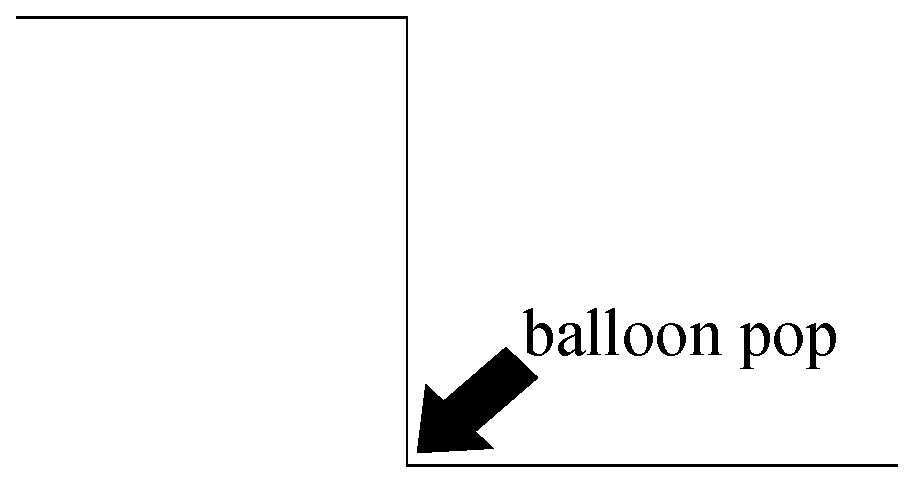
\epsfig{file=balloonpop.eps, height = 1.25in}
\caption{Balloon Pop - step excitation}
\end{center}


\end{minipage}
\begin{minipage}[b]{0.5\linewidth} 
\begin{center}
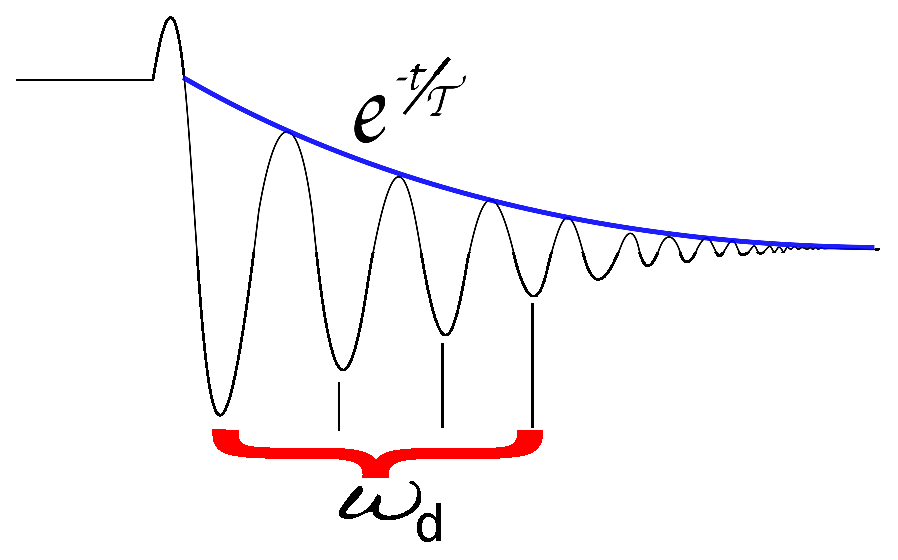
\epsfig{file=timedomain.eps, height=1.5in}
\caption{Time Domain - underdamped repsonse}
\end{center}

\end{minipage}
\end{figure}


\begin{figure}[htb]
\begin{center}
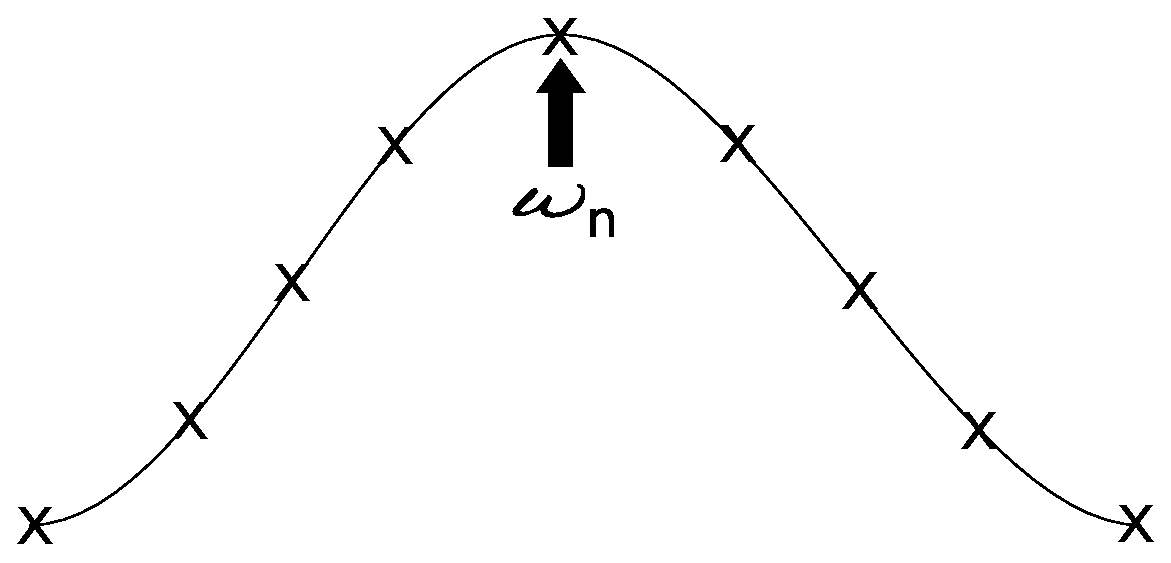
\epsfig{file=freqdomain.eps,height=1.25in}
\caption{Frequency Domain - underdamped response}
\end{center}
\end{figure}

From the frequency domain, the half-power bandwidth can be calculated from the -3 dB points ($\omega_2 - \omega_1$).

\begin{equation} \dfrac{\omega_2 - \omega_1}{\omega_n} = 2\zeta = \dfrac{1}{Q} \end{equation}

{\bf Consider:} Step is broadband.  What about steady-state sinusoidal inputs?

\end{document}
